\documentclass{article}

\usepackage{graphicx}
\usepackage[left=2cm, right=2cm, top=2cm]{geometry}

\begin{document}

% The following part of this document will be placed in the Methods section

The first test determines which coordinate system(s) and which version of the
derivation (general versus specific) ought to be used to produce the most
reliable results as the mass ratio decreases. This test is done for
the binary lens. In all cases, the two bodies are assumed to lie on the real
axis. The coordinate frames that are being considered are: the geometric center
frame, which assumes the vertical axis lies halfway between the star and the
planet; the planetary caustic frame, which assumes the central point of the
planetary caustic lies on the origin; the planet frame; the star frame; and
the center-of-mass frame. All calculations were done using the complex
polynomial root solver in Skowron and Gould 2012, for a constant value of s.

To test the success of each calculation, I simulated a grid of coordinates
in the source plane, centered on the planetary caustic. At each point, I
calculated the number of images that should be produced if the source were
at that position. There should be three images when the source is outside
the caustic, and five images when the source is inside the caustic. I also
calculate the magnification at each of the points in the grid. These
simulations are done for each of the aforementioned coordinate frames, for
both the specifically-derived and general forms of the polynomial.

After making these plots, I checked whether they produced a result that
agrees with theoretical expectations, using a pass-or-fail determination.
This can be qualified visually, as it is clear when a method fails because the
plot will reproduce a very noisey result with seemingly no regard to the
caustic. \textbf{Figure 1} and \textbf{Figure 2} show the plots of the
number of accepted images; \textbf{Figure 3} and \textbf{Figure 4} show
the plots of the magnification for the same grid of points.

\begin{figure}
	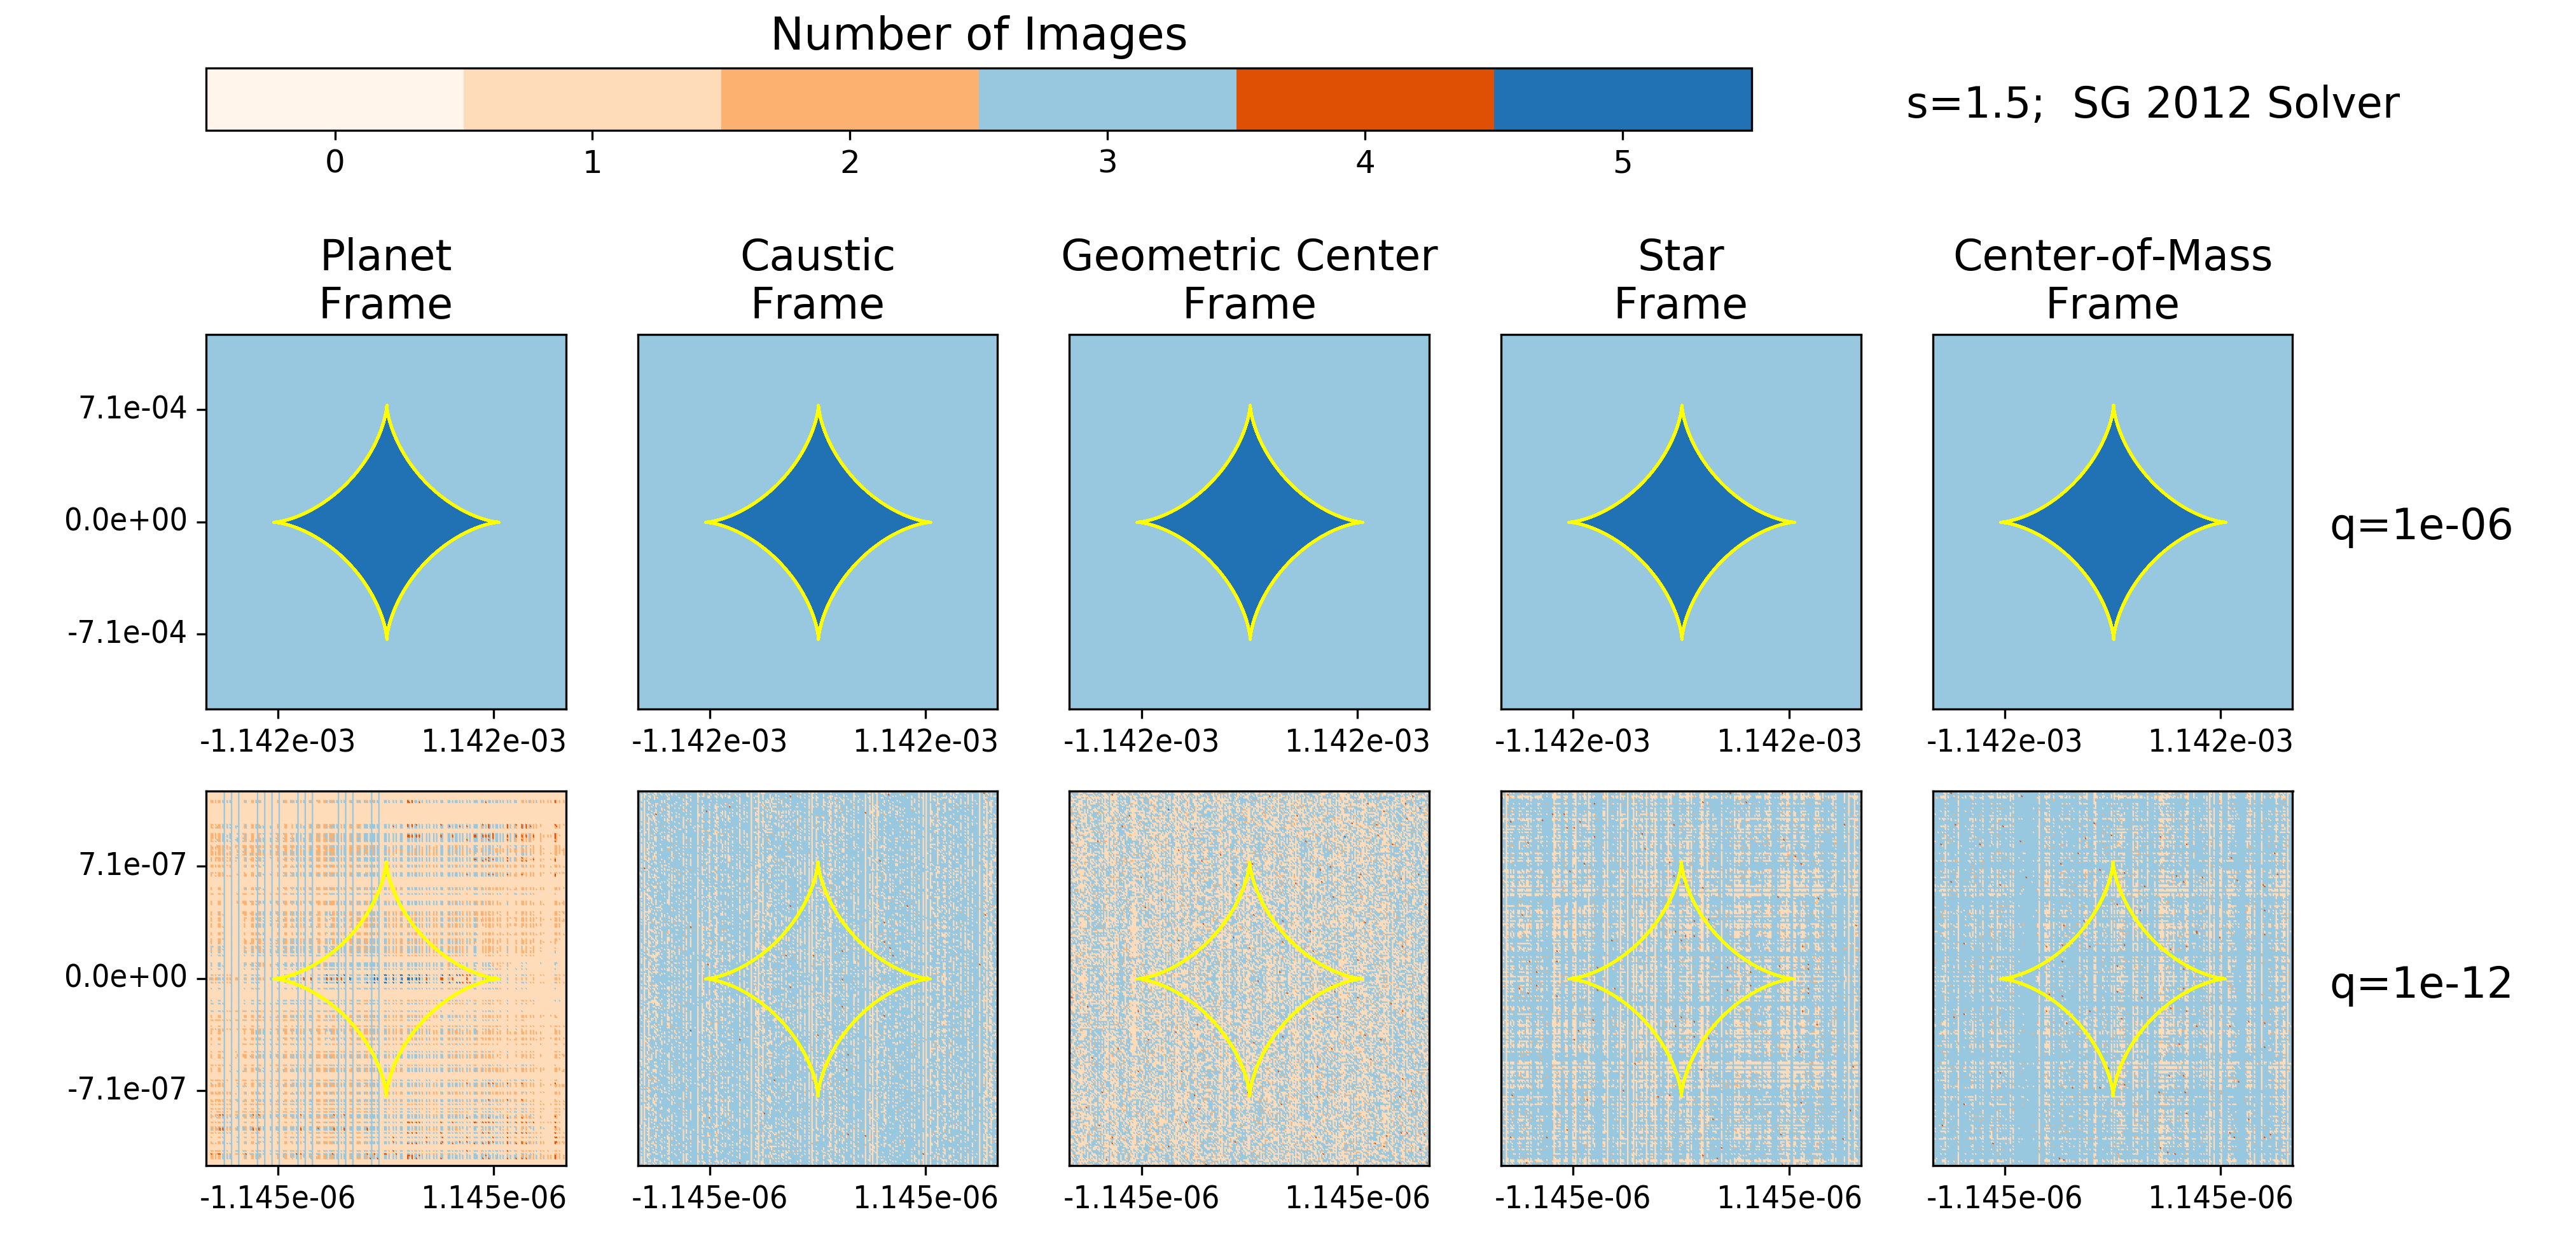
\includegraphics[width=0.9\textwidth]{../Tables/images_origin_0.png}
	\caption{The number of images versus position for each coordinate
	frame using the general form of the polynomial. The top row shows
	the plots for a mass ratio, $q=10^{-6}$. The bottom row shows the
	plots for a mass ratio, $q=10^{-12}$. Notice that the scale on the
	x- and y-axes scale by orders of magnitude, an effect of the two
	given mass ratios. As expected, for $q=10^{-6}$, the plots show the
	correct number of images for each coordinate system. However, for
	$q=10^{-12}$, the plots fail for all coordinate frames.}

	\vspace*{\floatsep}

	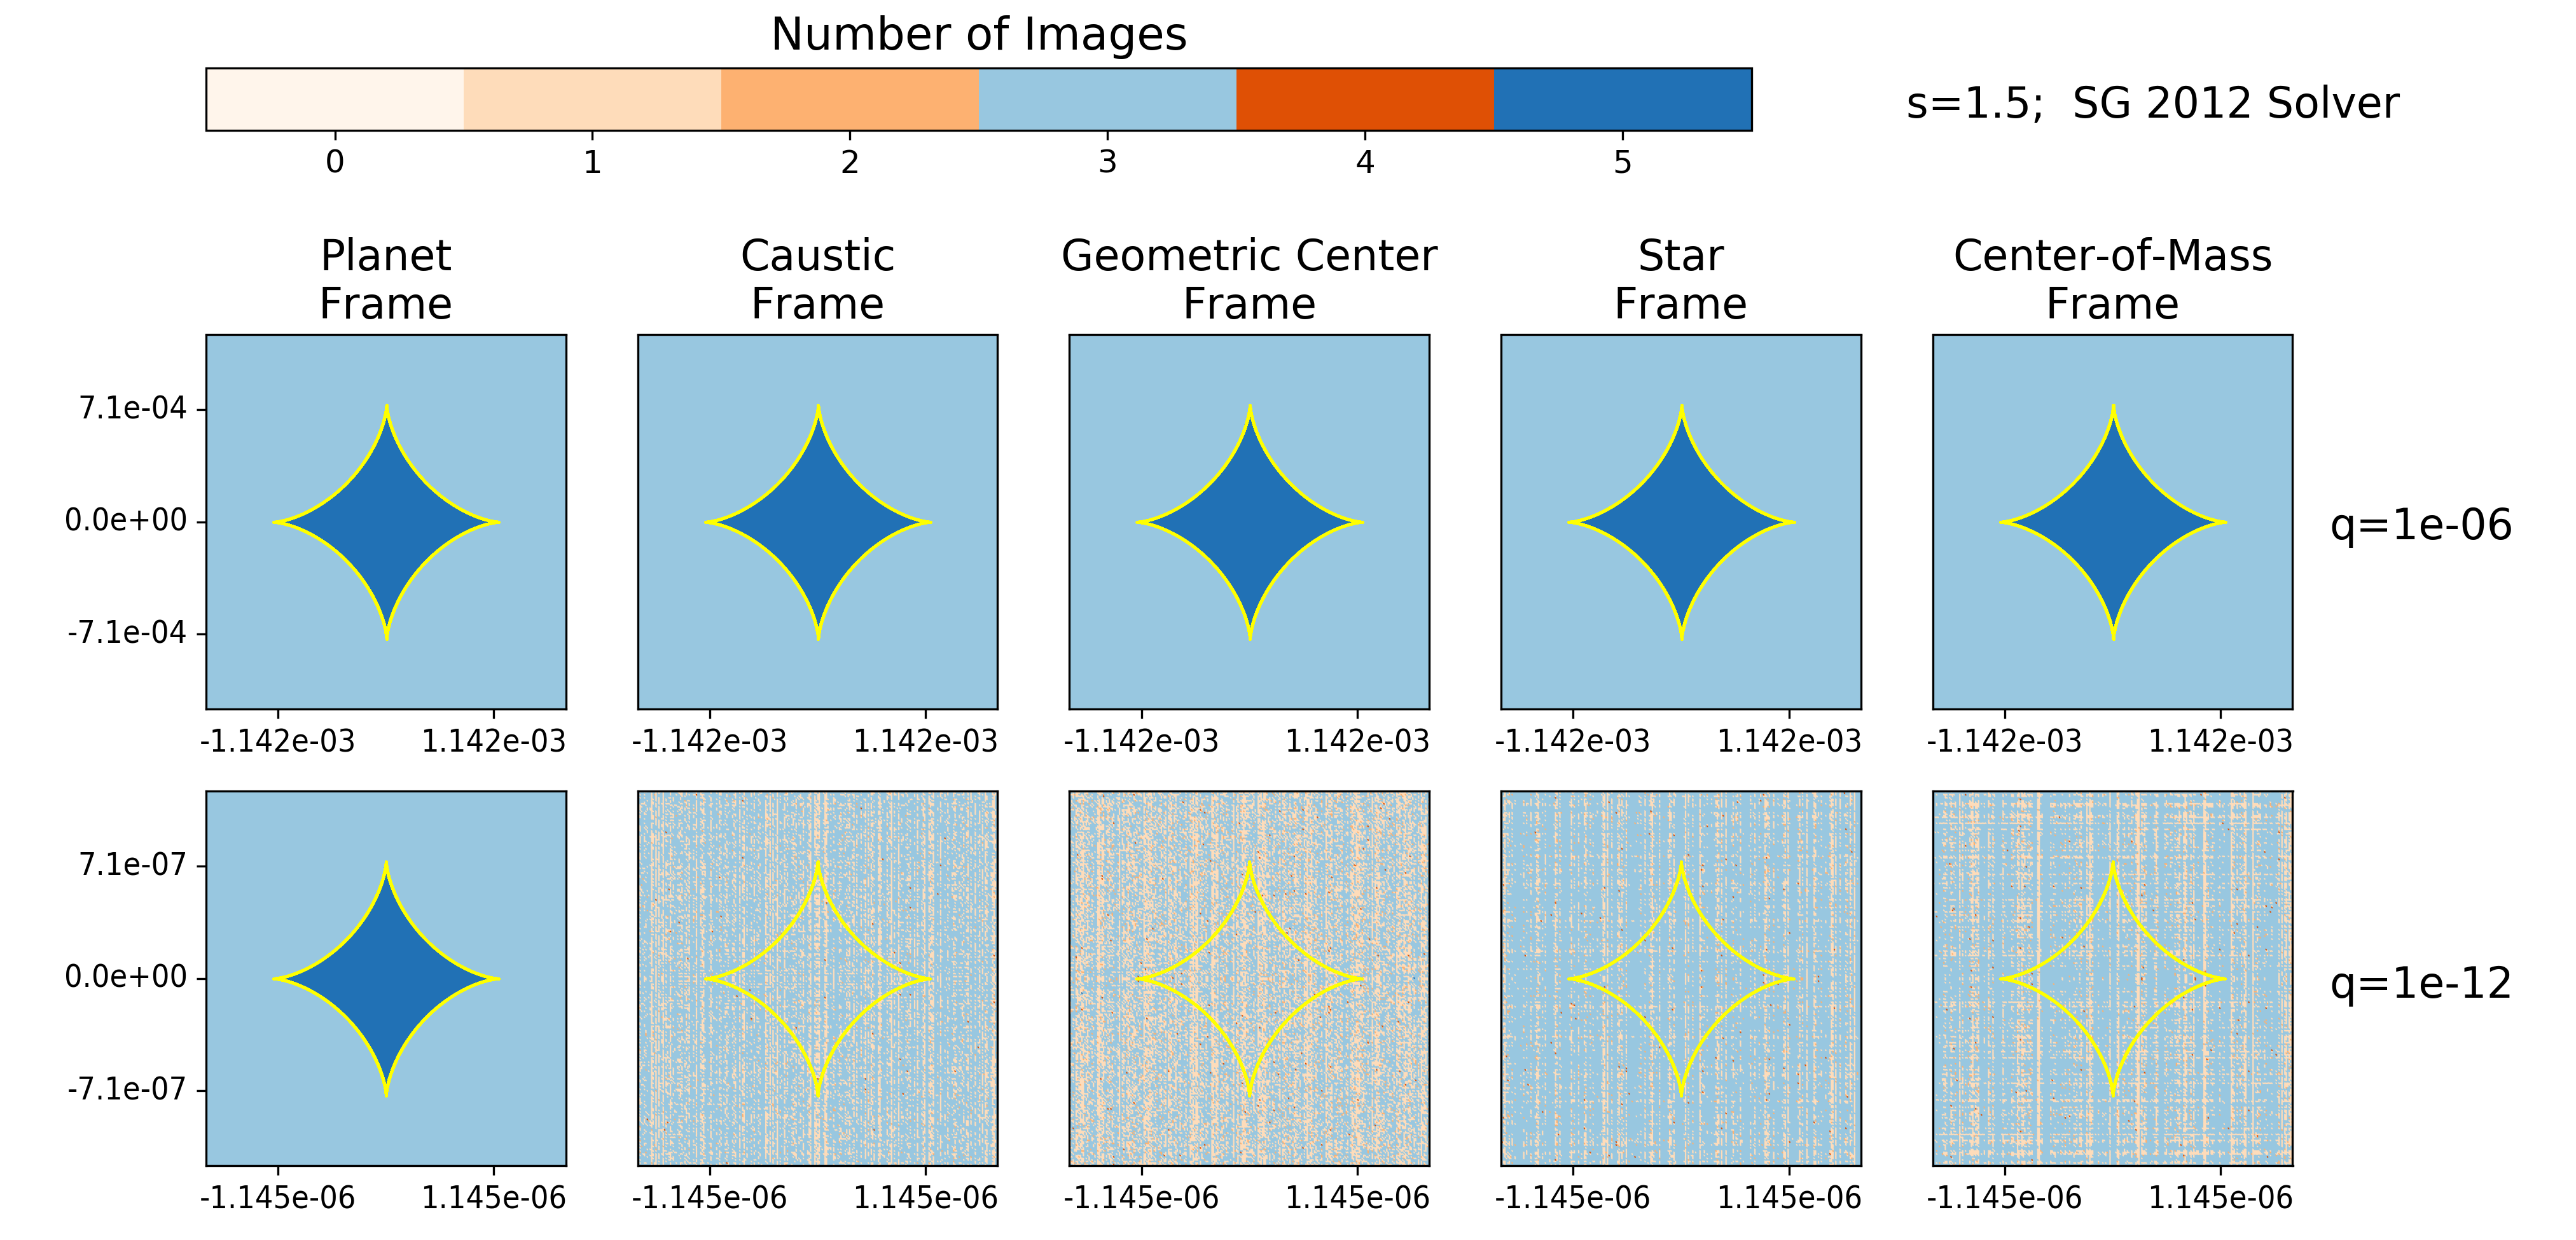
\includegraphics[width=0.9\textwidth]{../Tables/images_origin_1.png}
	\caption{Same as \textbf{Figure 1} except using the specifically-
	derived forms of the polynomial. As	expected, for $q=10^{-6}$, the
	plots show the correct number of images for each coordinate system.
	For $q=10^{-12}$, the plots fail for all coordinate frames except for
	the planet frame.}
\end{figure}

\begin{figure}
	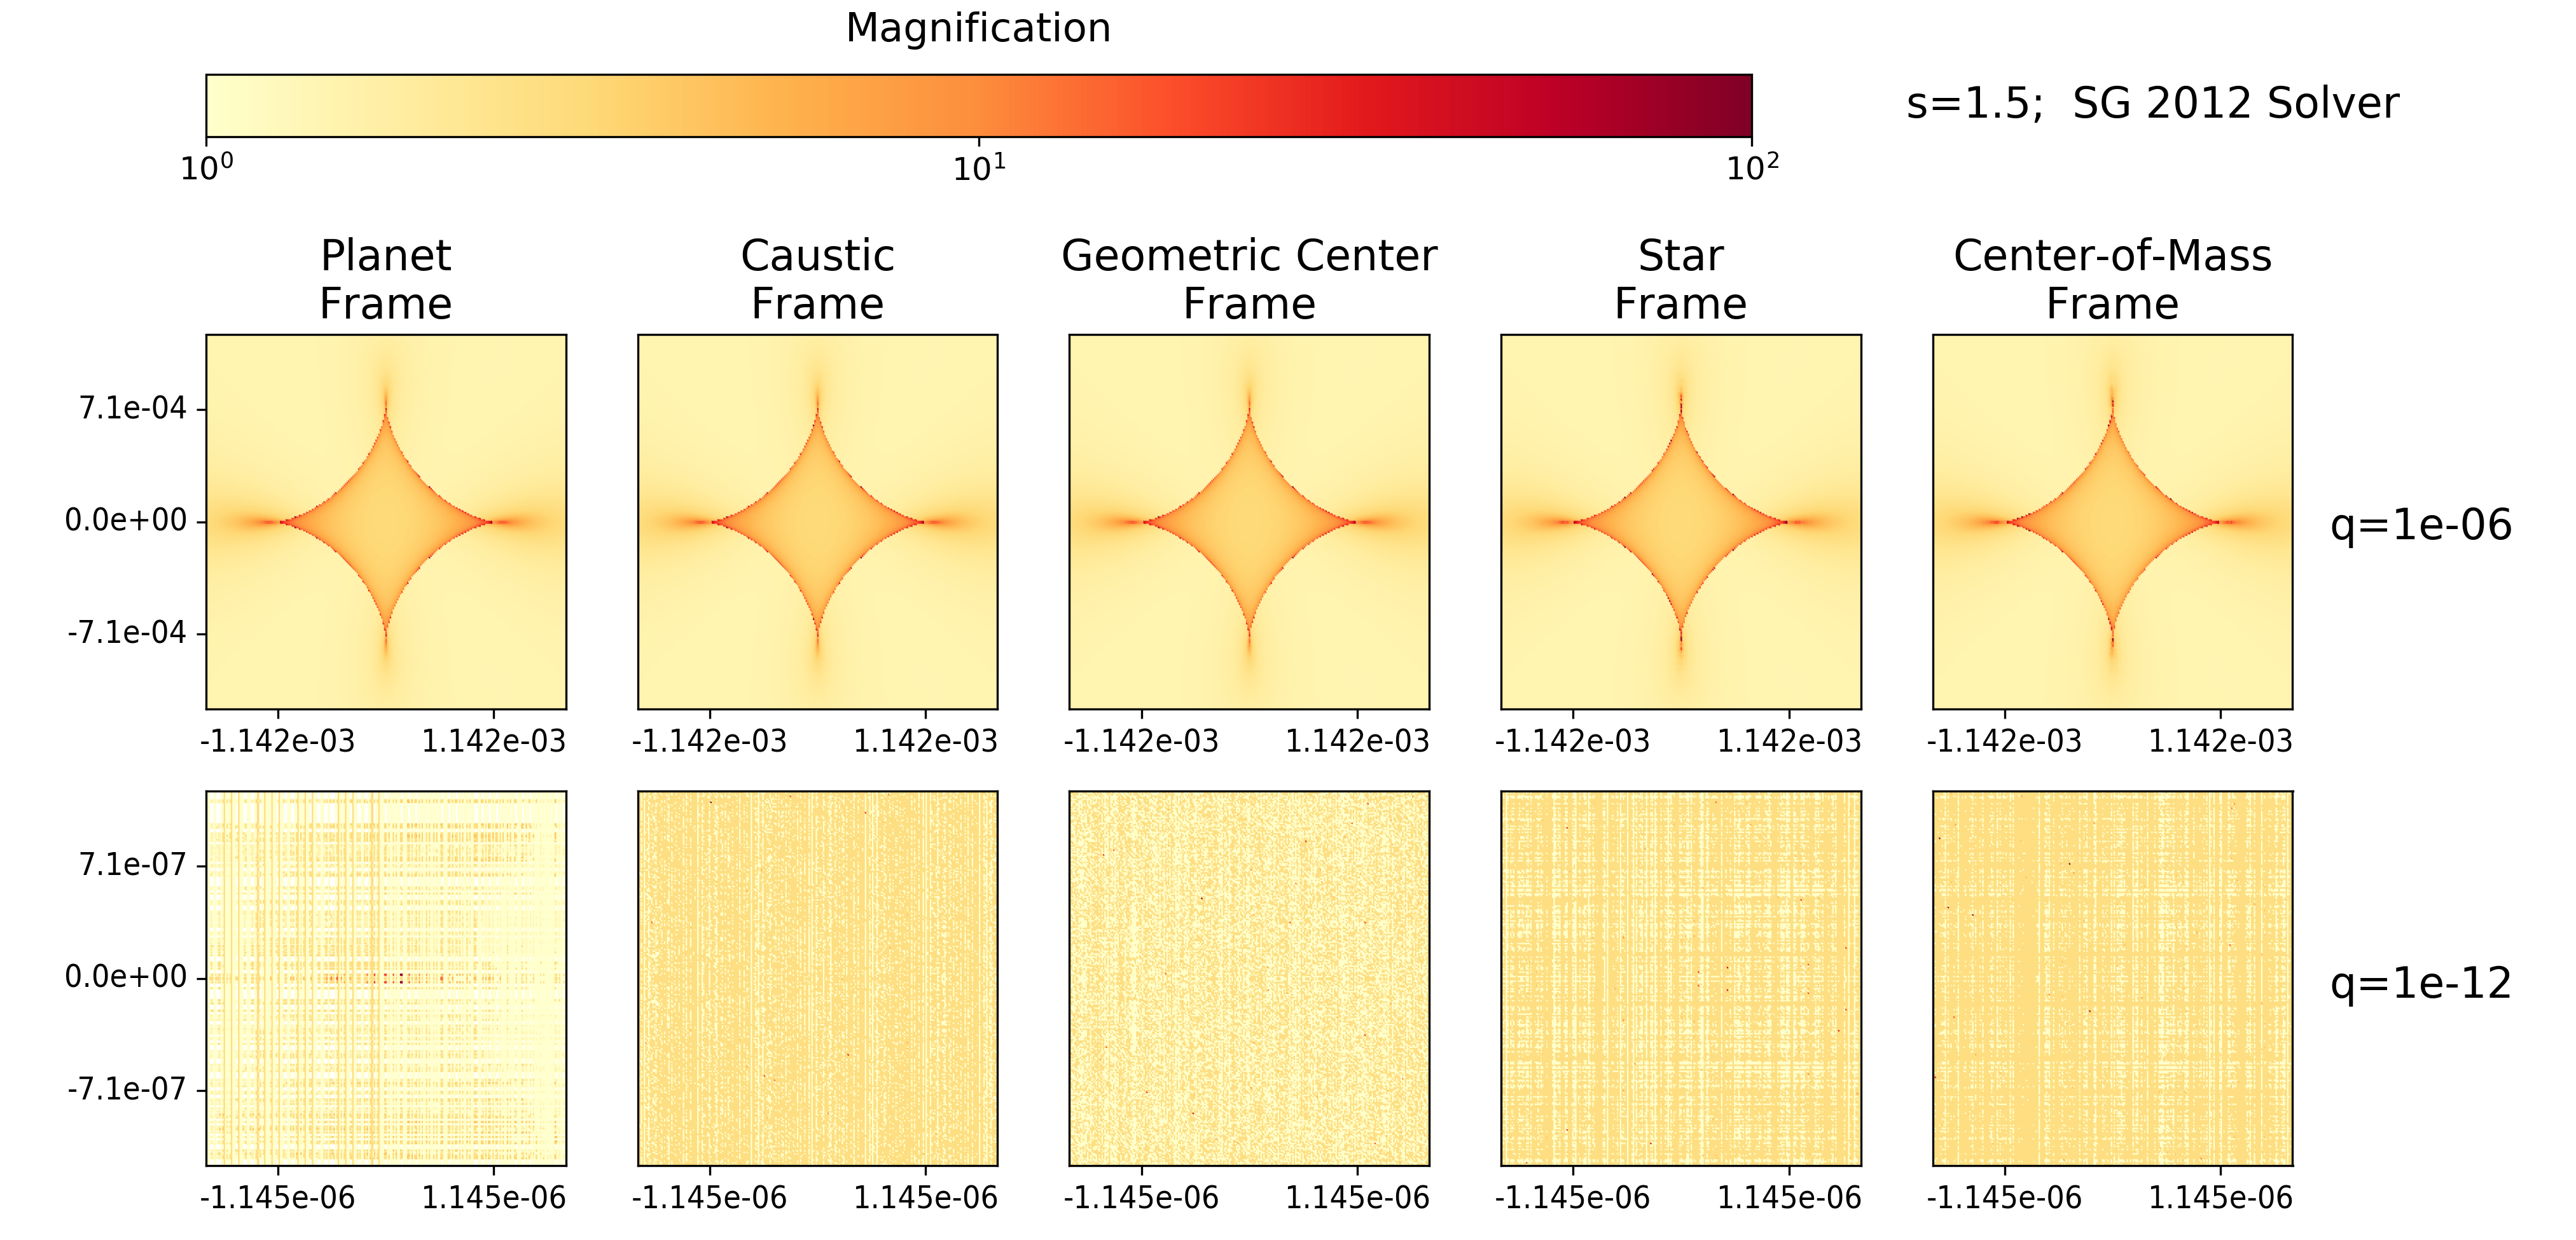
\includegraphics[width=0.9\textwidth]{../Tables/magn_origin_0.png}
	\caption{The magnification versus the position for each coordinate
	frame using the general form of the polynomial. As seen in plots
	of the number of images, the simulations pass for all coordinate
	frames when $q=10^{-6}$, and fail for all coordinate frames when
	$q=10^{-12}$.}

	\vspace*{\floatsep}

	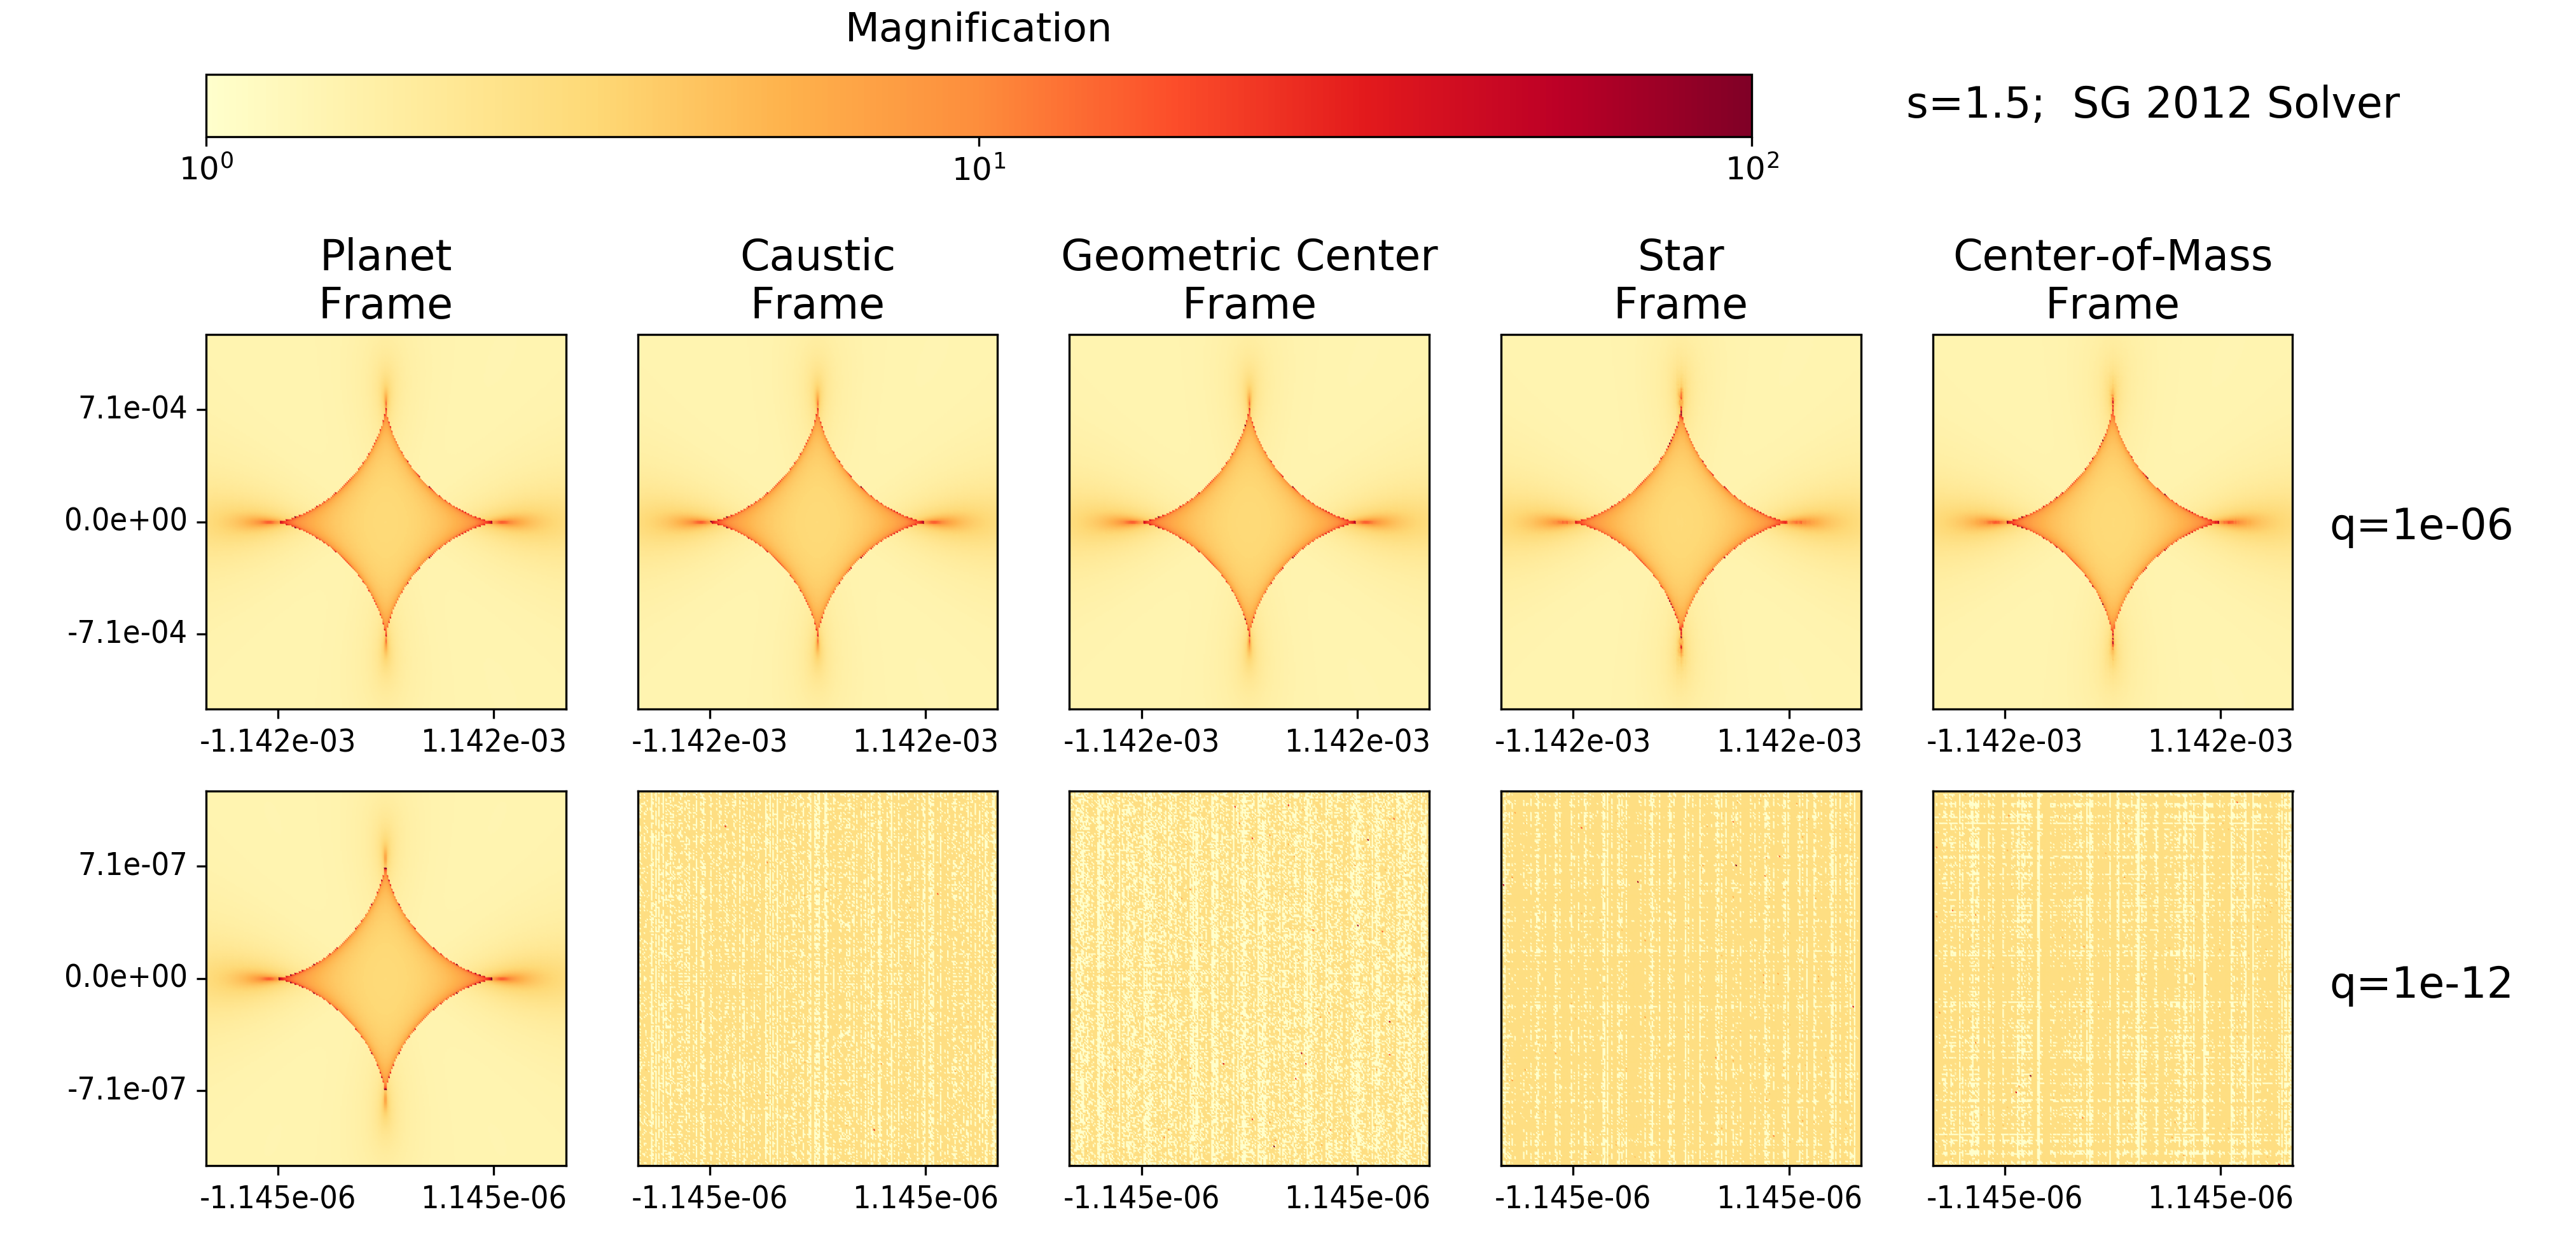
\includegraphics[width=0.9\textwidth]{../Tables/magn_origin_1.png}
	\caption{Same as \textbf{Figure 3} except using the specifically-
	derived forms of the polynomial. As seen in the plots of the number
	of images, when $q=10^{-12}$, the simulation fails for all coordinate
	frames except for the planet frame.}
\end{figure}

% The following part of this document will be placed in the Results/Analysis
% section

When using the general form of the polynomial equation, the planet frame
performs slightly better than the other frames as the mass ratio approaches
$10^{-8}$. At mass ratios greater than $10^{-7}$, none of the coordinate
frames produce any errors. However, all of the frames result in high numbers
of errors when the mass ratio drops below something of the order $10^{-8}$.

On the other hand, when using the specifically-derived forms of the polynomial,
the planet frame produces a correct plot of the number of images all the way
down to a mass ratio of $10^{-15}$; whereas the other frame fail. The
speculated reason for this is that the form of the polynomial specifically
derived for the planet frame elimates all instances of the term, $q^{2}$;
whereas the derivations for all other frames have at least one $q^{2}$ term.
Because 64-bit floating point numbers can only store around 16 digits, many
errors tend to accumulate when adding terms of the order $10^{0}$ with other
terms of the order $10^{-16}$. By eliminating every instance of $q^{2}$,
it is possible to keep every significant digit throughout the calculation with
mass ratios all the way down to $10^{-15}$.

\end{document}
